%http://mcclinews.free.fr/latex/beamermodif/beamerbox.html
\documentclass[9pt]{beamer}

\usepackage[utf8]{inputenc}
\usepackage[T1]{fontenc}
\usepackage[french]{babel}
\usepackage{fontspec}
\usepackage{csquotes}
\usepackage{subcaption}
\usepackage[backend=biber,style=authoryear,sorting=none]{biblatex}
\usepackage{capt-of}% caption in column envs
\usepackage{setspace}%line spacing

% colors
\definecolor{plum}{rgb}{0.44, 0.11, 0.11}
\definecolor{lilac}{rgb}{0.8, 0.8, 1.0}
\definecolor{pastelviolet}{rgb}{0.8, 0.6, 0.79}
\definecolor{moccasin}{rgb}{0.98, 0.92, 0.84}
\definecolor{darkterracotta}{rgb}{0.8, 0.31, 0.36}
\definecolor{lightmauve}{rgb}{0.86, 0.82, 1.0}
%\definecolor{sauge}{RGB}{148, 181, 215}
%\definecolor{sauge}{HTML}{DBD2DD}
%\definecolor{sauge}{HTML}{C4D0D3}
\definecolor{sauge}{HTML}{C2CED3}
\definecolor{darkdust}{RGB}{83, 52, 89}

% style the beamer template
\usecolortheme{sauge}
\usefonttheme{serif}
\usetheme{Goettingen}
\makeatletter
\setbeamertemplate{sidebar canvas \beamer@sidebarside}[default]

%\setbeamertemplate{navigation symbols}{}
\setbeamertemplate{items}[square]
\setbeamertemplate{sections/subsections in toc}[square]
\makeatother

% captions
\usepackage{subcaption}
\usepackage{caption}
\DeclareCaptionFormat{custom}{%
	\scriptsize{#1#2#3}
}
\captionsetup{format=custom,width=0.8\textwidth}
\captionsetup[listing]{skip=-10pt}

% tikz
\usepackage{tikz}
\usetikzlibrary{shapes.geometric}

\tikzstyle{act} = [%
	draw,%
	rectangle,%
	rounded corners=3pt,%
	minimum height=1cm,%
	fill=lilac,%
	draw=plum,%
	text centered,%
	text width=4cm%
]
\tikzstyle{db} = [%
	cylinder,%
	shape border rotate=90,%
	aspect=0.25,%
	fill=pastelviolet,%
	draw=plum,%
	text centered,%
	text width=4cm%
]
\tikzstyle{arrow} = [%
	thick,%
	->,%
	>=stealth,%
	color=plum%	
]
\tikzstyle{doublearrow} = [%
	thick,%
	<->,%
	>=stealth,%
	color=plum,%
]
\pgfdeclarelayer{bg}    % declare background layer
\pgfsetlayers{bg,main}  % set the order of the layers (main is the standard layer)

% commands
\newcommand{\emulatecaption}[1]{%
	% emulate the `\caption` style outside of `figure` env
	\begin{spacing}{0.9}%
		\scriptsize F\textsc{igure} -- #1%
	\end{spacing}
}
\newcommand{\tikztemplate}[2]{%
	% template for our tikz elements
	% #1: title
	% #2: inner content
	\texttt{\textsc{#1}}
	\\~\\
	\begin{spacing}{0.9}
		\small{#2}
	\end{spacing}
}

\title[\enquote{La marque du lieu} dans le \enquote{quartier Richelieu}]{\enquote{La marque du lieu} dans le \enquote{quartier Richelieu}}
\subtitle{Implications de la notion de lieu pour la modélisation et la visualisation d'un corpus iconographique, cartographique et textuel (Paris, 1750-1950)}
\author[P. Kervegan, C. Duvette, C. Prudhomme, C. Jeanson \textit{et. al.}]{%
	Paul Kervegan\textsuperscript{1}
	\and Charlotte Duvette\textsuperscript{1}\\
	\and Colin Prudhomme\textsuperscript{1}
	\and Loïc Jeanson\textsuperscript{2}
	\and Justine Gain\textsuperscript{1}
	\and Esther Dasilva\textsuperscript{1}
	\and Louise Baranger\textsuperscript{1}
	\\~\\
	\textsuperscript{1}: Institut national d'histoire de l'art (France)\\
	\textsuperscript{2}: Université de Lausanne (Suisse)
}
\date{Conférence Humanistica, 27 juin 2023, Genève}

\usepackage{hyperref}
\hypersetup{
	%colorlinks=true,
	%linkcolor=darkdust,
	citecolor=wildstrawberry,      
	urlcolor=wildstrawberry,
	pdfauthor={Paul KERVEGAN and Charlotte Duvette and Colin Prudhomme and Loïc Jeanson and Justine Gain and Esther Dasilva and Louise Baranger}, 
	pdftitle={\enquote{La marque du lieu} dans le \enquote{quartier Richelieu}: Implications de la notion de lieu pour la modélisation et la visualisation d'un corpus iconographique, cartographique et textuel (Paris, 1750-1950)}, 
	pdfsubject={Modélisation de données, géohistoire},
	pdfkeywords={modélisation}{géohistoire}{histoire de l'architecture}{sql}{modélisation 3D}{postgresql}{sig}{système d'information géographique}
}

\begin{document}
% present the outline at search section change
\AtBeginSection{
	\begin{frame}{Plan}
		\tableofcontents[currentsection]
	\end{frame}
}

\begin{frame}
	\titlepage
\end{frame}

%\begin{frame}{title}{subtitle}
\begin{frame}{Plan}
	\tableofcontents
\end{frame}

\section{Aborder un quartier par le lieu}
\subsection{La topographie du quartier Richelieu}
\begin{frame}{Aborder un quartier par le lieu}{La topographie du quartier Richelieu}
	\begin{figure}[h]
		\centering
		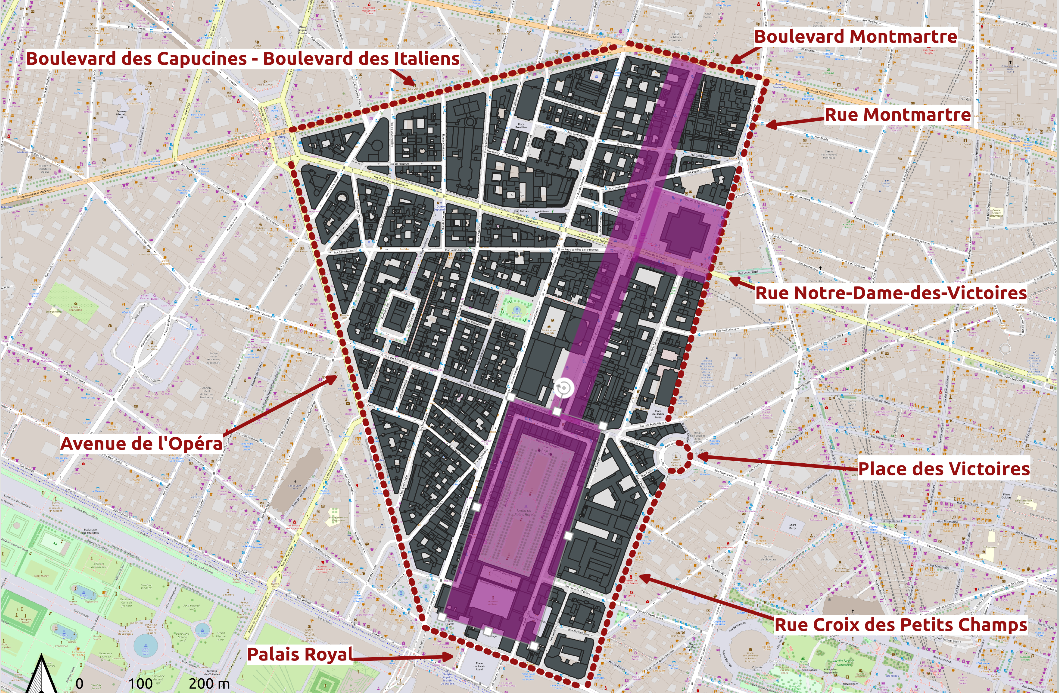
\includegraphics[width=\textwidth]{includes/topographie.png}
		\caption{La topographie du quartier Richelieu}
	\end{figure}
\end{frame}

\subsection{Qu'est-ce qui fait quartier au XIX\textsuperscript{e} siècle?}
\begin{frame}{Aborder un quartier par le lieu}{Qu'est-ce qui fait quartier au XIX\textsuperscript{e} siècle?}
	\begin{figure}
		\centering
		\begin{subfigure}{0.7\textwidth}
			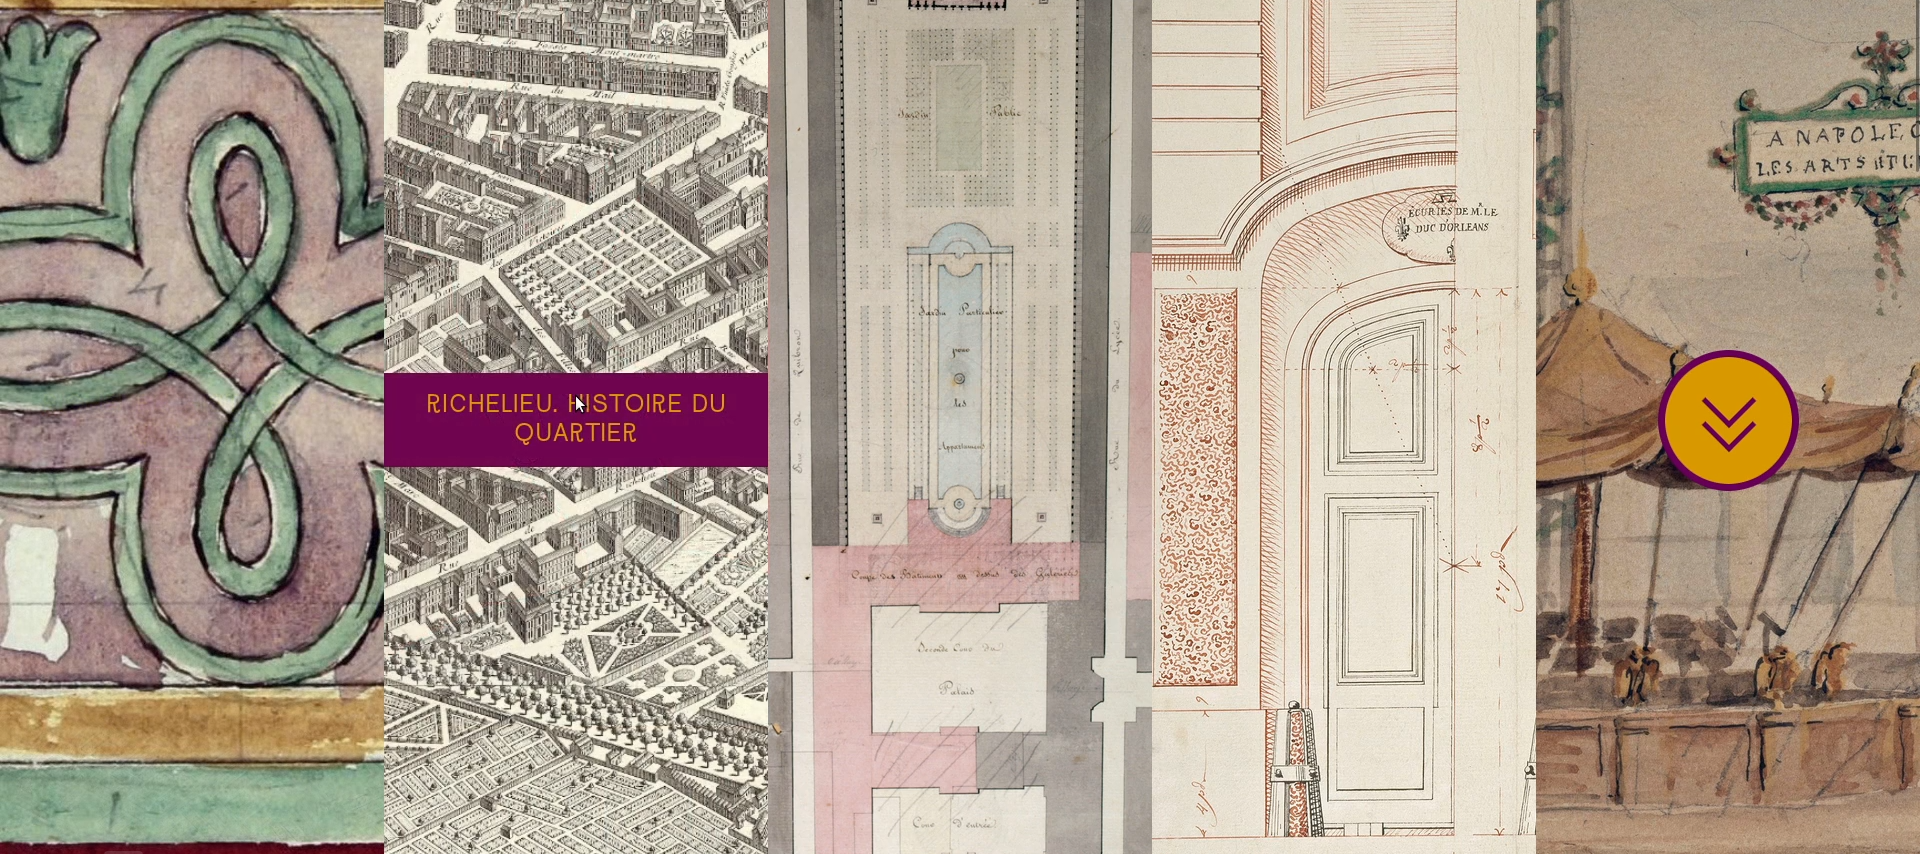
\includegraphics[width=\textwidth]{includes/app_1.png}
		\end{subfigure}
		\begin{subfigure}{0.7\textwidth}
			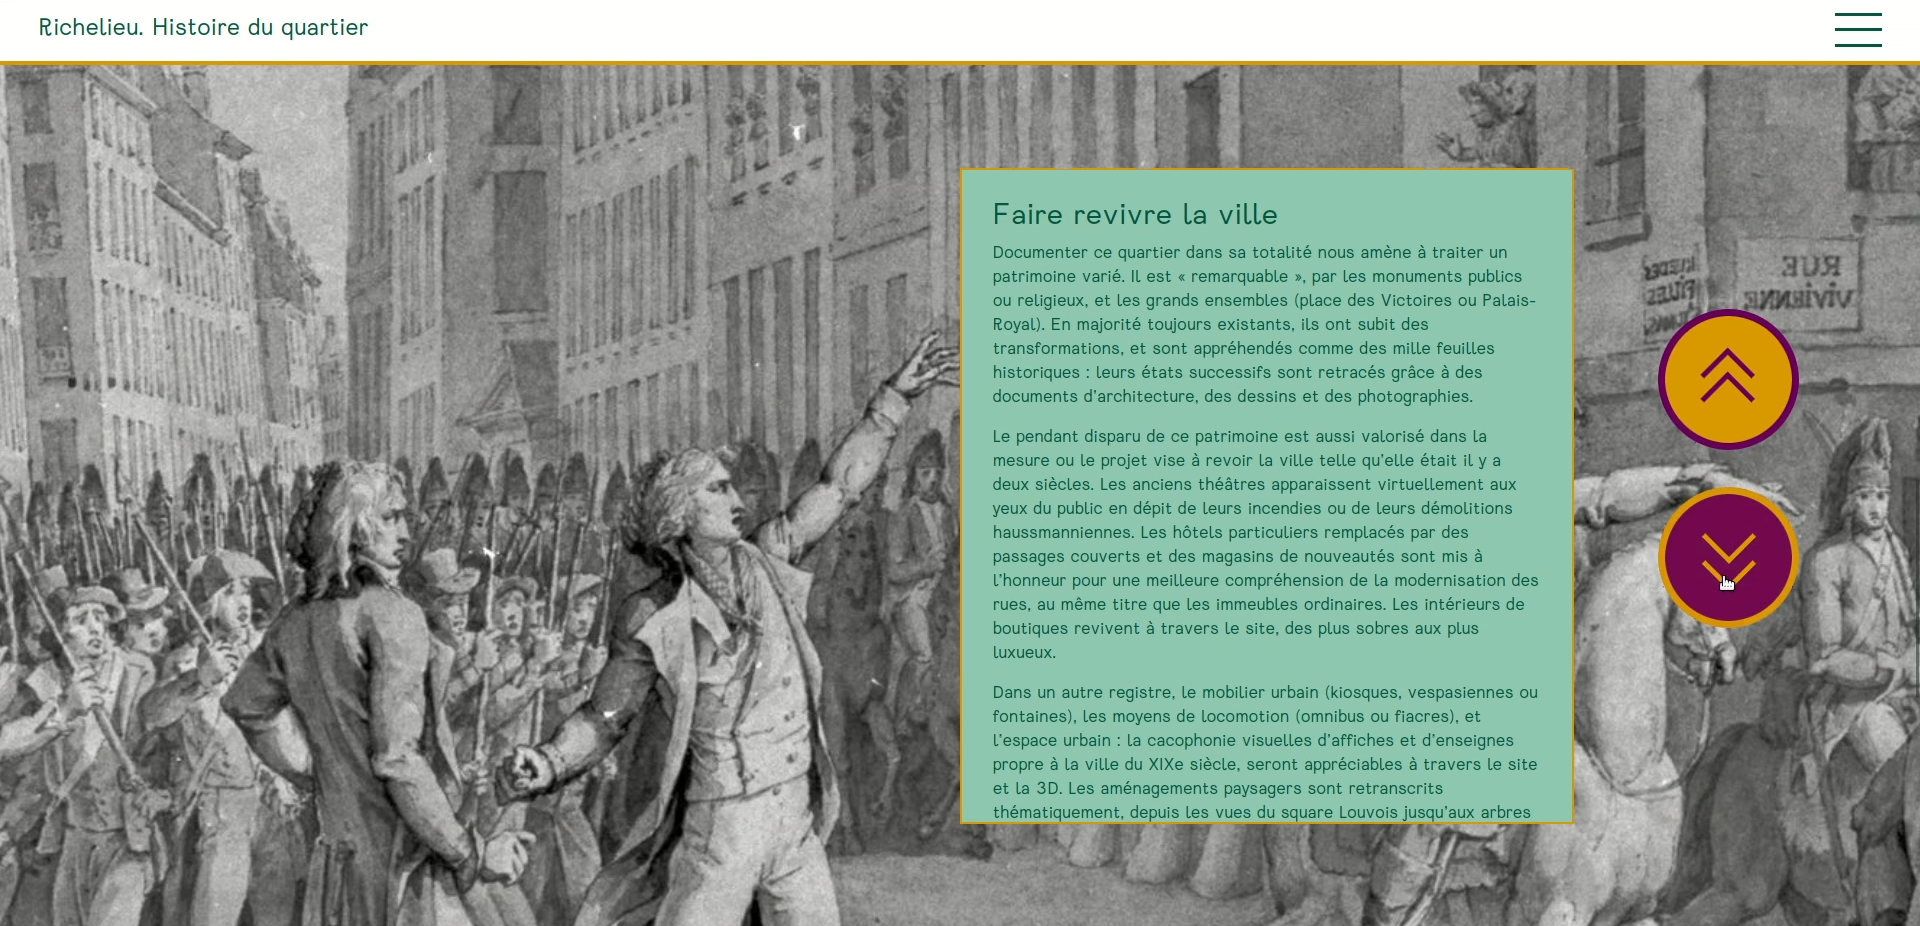
\includegraphics[width=\textwidth]{includes/app_2.png}
		\end{subfigure}
		\caption{Deux captures d'écran de l'application Web du projet \enquote{Richelieu}}
	\end{figure}
\end{frame}

% 2e slide appli

\subsection{Problématiques}
\begin{frame}{Aborder un quartier par le lieu}{Les réseaux du quartier}
	\begin{columns}[c]
		\begin{column}{0.5\textwidth}
			\begin{tabular}{p{\textwidth}}
				\begin{figure}
				\centering
					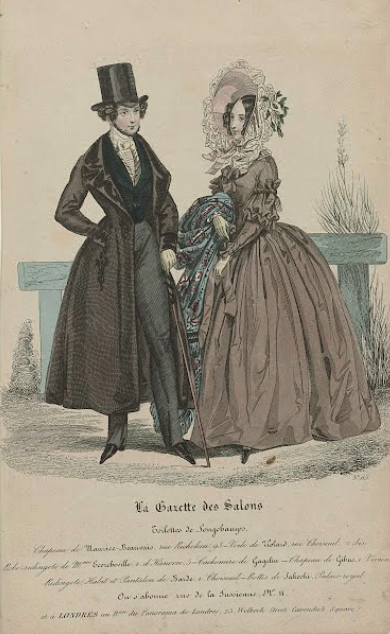
\includegraphics[width=0.7\textwidth]{includes/costume.png}
				\end{figure}
				\\ 
				\emulatecaption{La Gazette des Salons, 1836, n°115, Toilettes de Longchamp, Rijksmuseum, Amsterdam}
			\end{tabular}
		\end{column}
		\begin{column}{0.5\textwidth}
			\begin{itemize}
				\item Chapeau de Maurice-Beauvais, \textbf{93 rue Richelieu}
				\item Redingote habit et pantalon de Barbe, \textbf{Rue Choiseul}
				\item Bottes de Sakoski, \textbf{Palais-Royal}
				\item Chapeau de Gibus, \textbf{Rue Vivienne}
				\item Voile de Violard, \textbf{2 bis rue Choiseul}
				\item Robe-redingote de Mme Ecorcheville, \textbf{5 rue d’Hanovre}
			\end{itemize}		
		\end{column}
	\end{columns}
\end{frame}

\begin{frame}{Aborder un quartier par le lieu}{Les réseaux du quartier}
	\begin{figure}
		\centering
		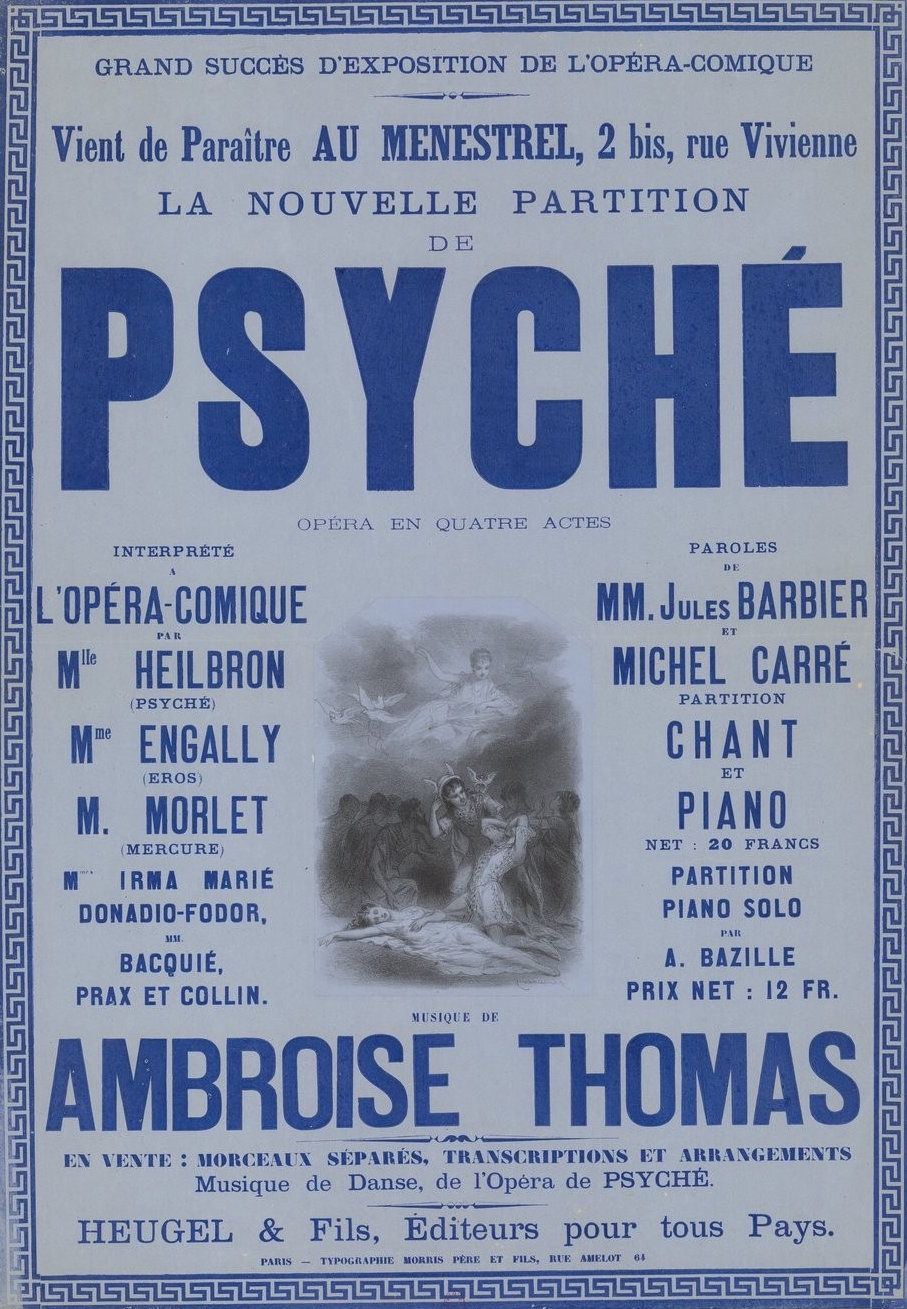
\includegraphics[height=0.65\textheight]{includes/psyche.png}
		\caption{\textit{Psyché. Opéra en quatre actes, interprété à l'Opéra–Comique...}, affiche, lithographie de Antonin-Marie Chatinière, 1878, Département bibliothèque-musée de l’Opéra, BnF. Publicité pour des imprimés en vente au \textbf{Au Ménestrel, 2 bis, rue Vivienne}}
	\end{figure}
\end{frame}

\begin{frame}{Aborder un quartier par le lieu}{Les réseaux du quartier}
	\begin{figure}
		\centering
		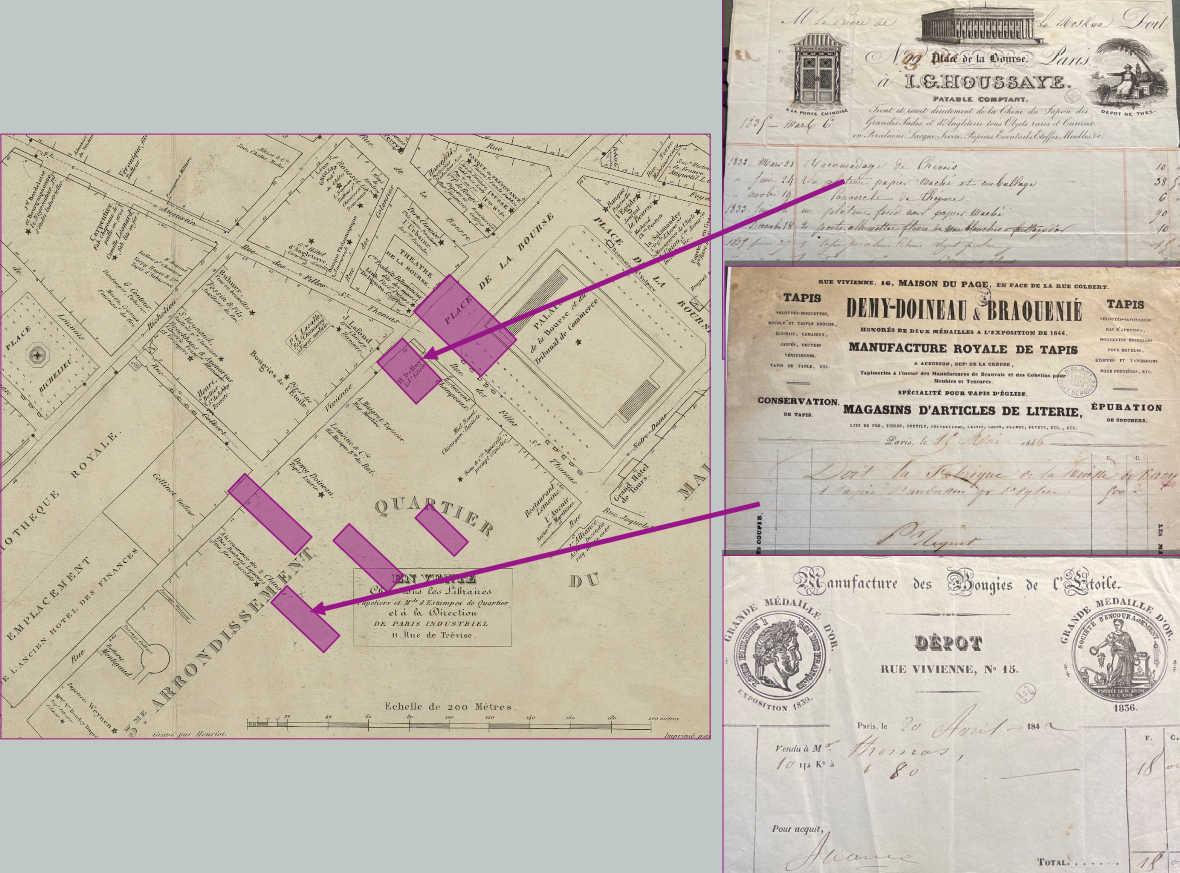
\includegraphics[width=0.9\textwidth]{includes/spatial0.png}
		\caption{Spatialisation de sources archivisitiques}
	\end{figure}
\end{frame}

\begin{frame}{Aborder un quartier par le lieu}{Histoire des mentalités}
	\begin{columns}[c]
		\begin{column}{0.5\textwidth}
			\begin{tabular}{p{\textwidth}}
				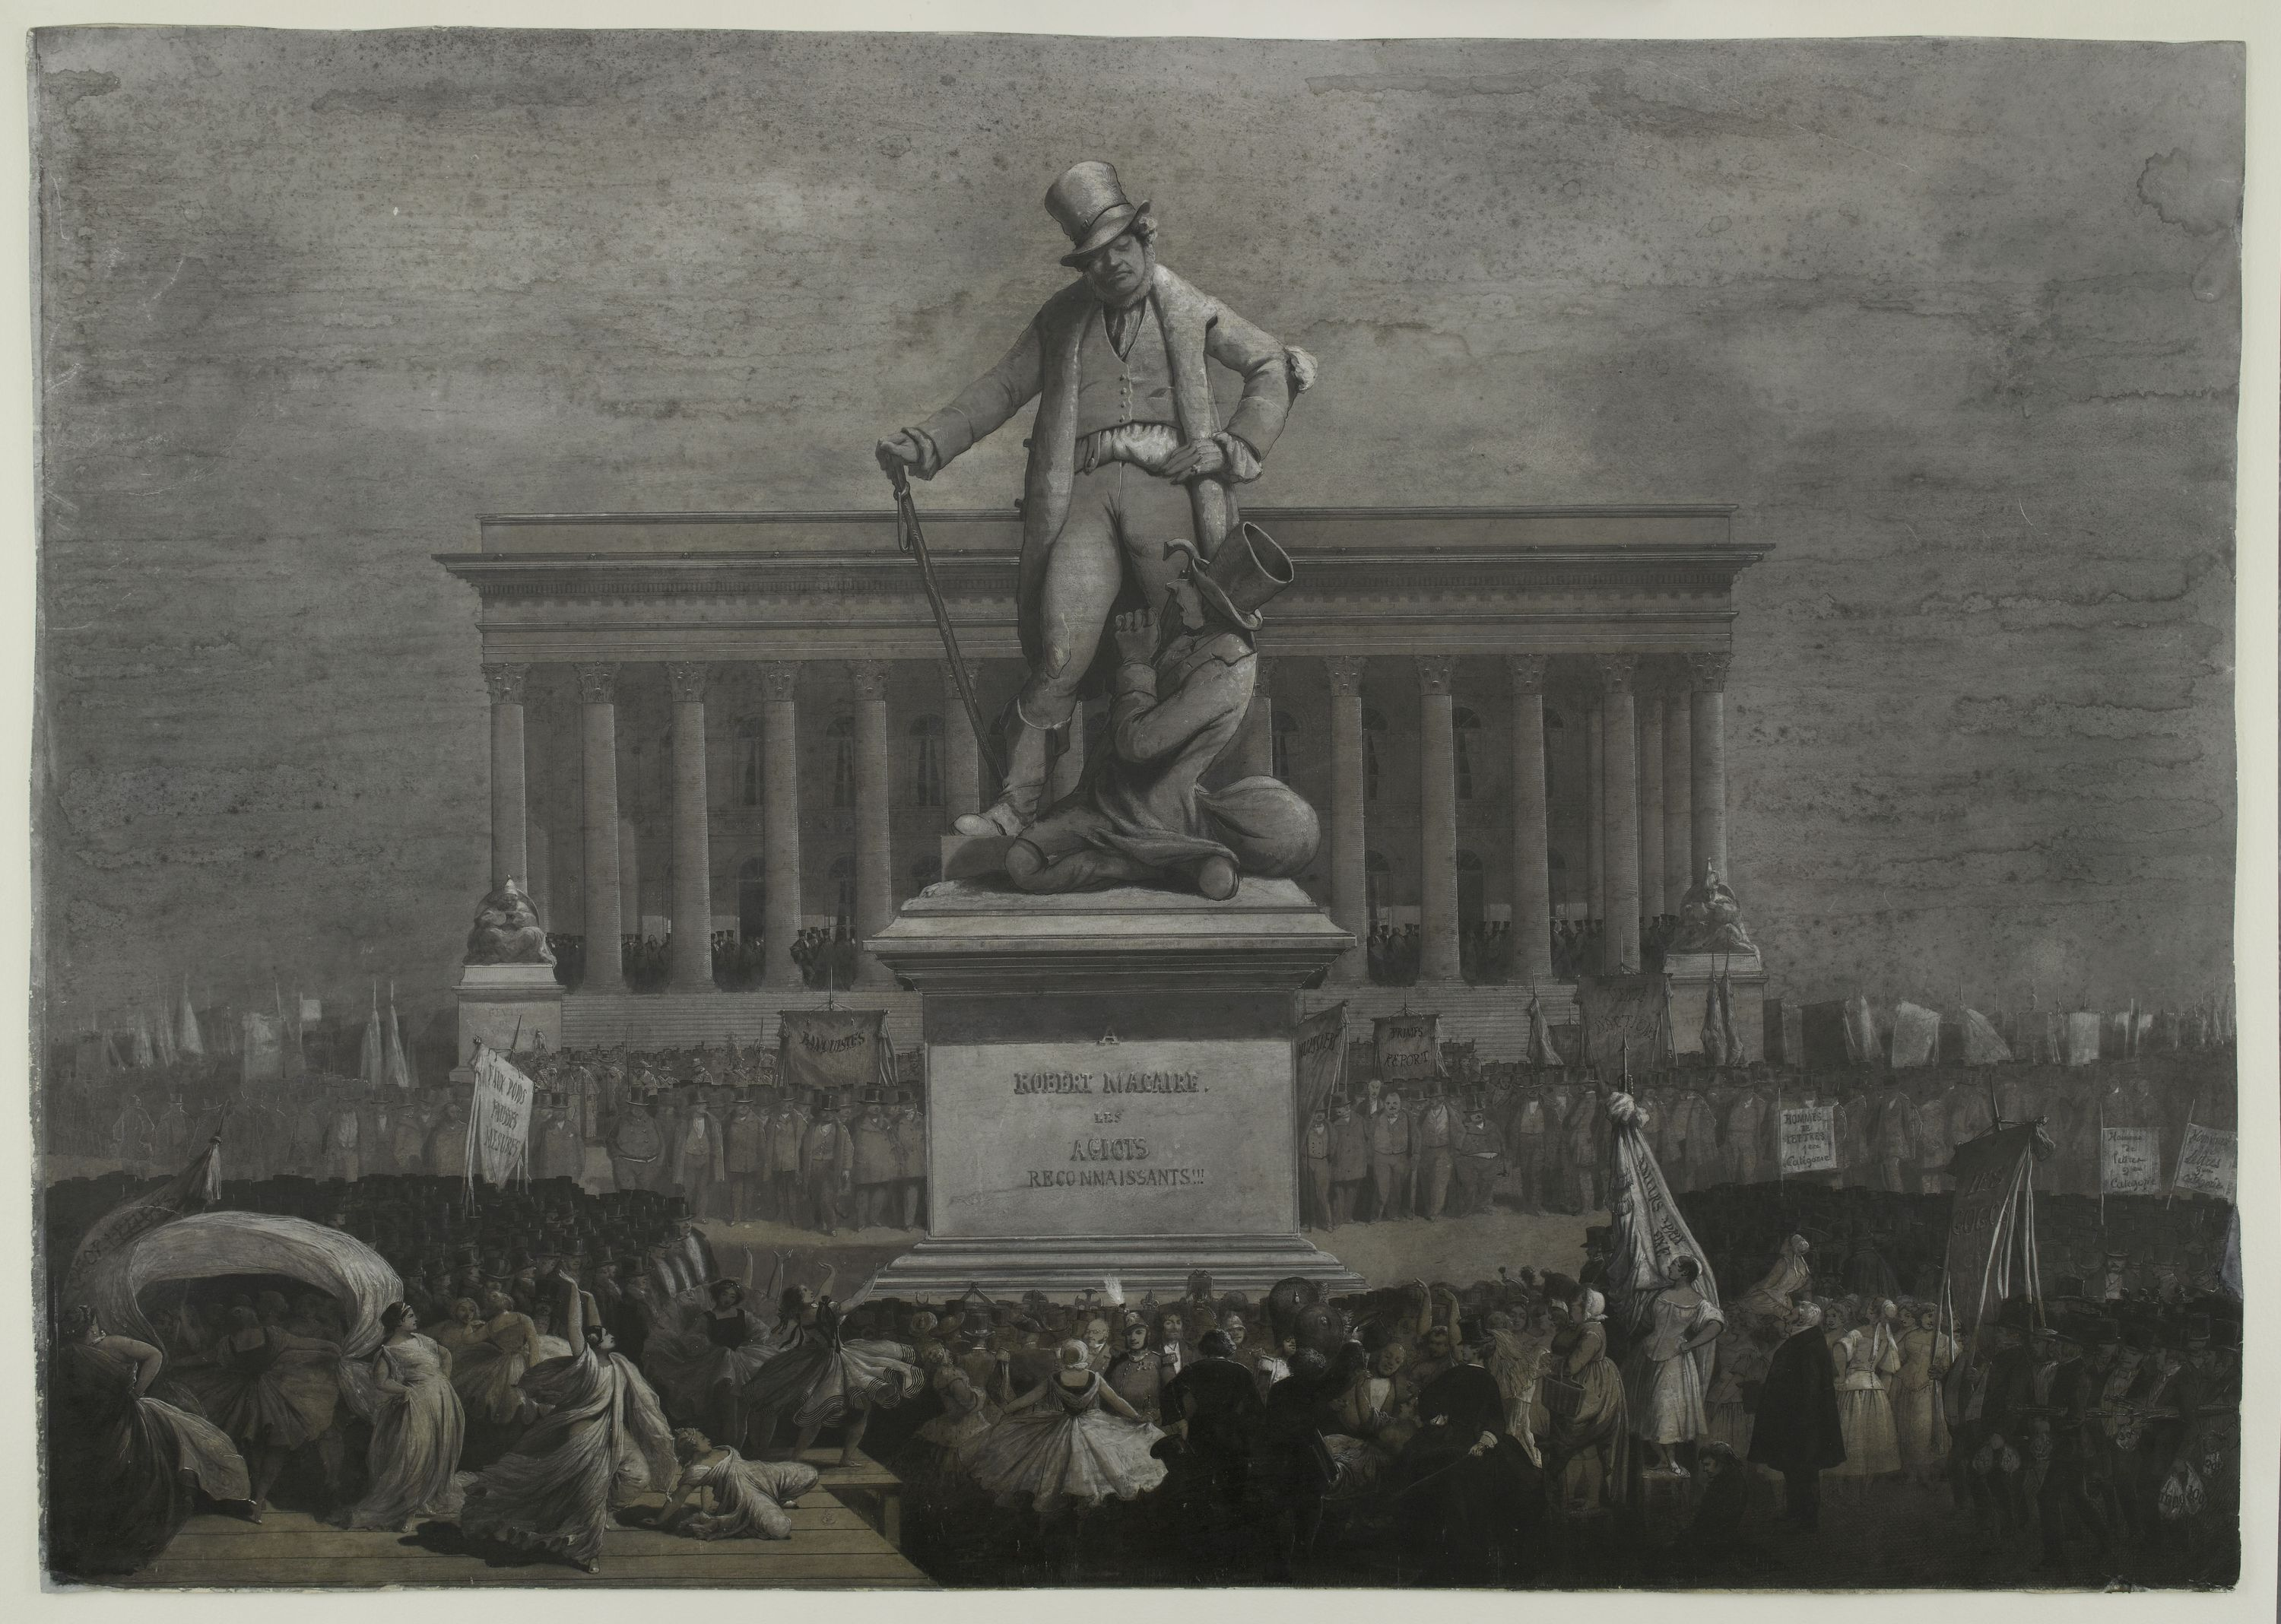
\includegraphics[height=0.27\textheight]{includes/macaire.jpg}
				\\
				\emulatecaption{Lorentz, Alcide Joseph, \textit{Monument à Robert Macaire},1856, musée Carnavalet}
				\\
				\includegraphics[height=0.27\textheight]{includes/promenade.png}
				\\
				\emulatecaption{Jean-Baptiste Arnout, \textit{Promenade pittoresque dans Paris, n° 21}, musée Carnavalet}
			\end{tabular}
		\end{column}
		\begin{column}{0.5\textwidth}
			\begin{tabular}{p{\textwidth}}
				\begin{center}
					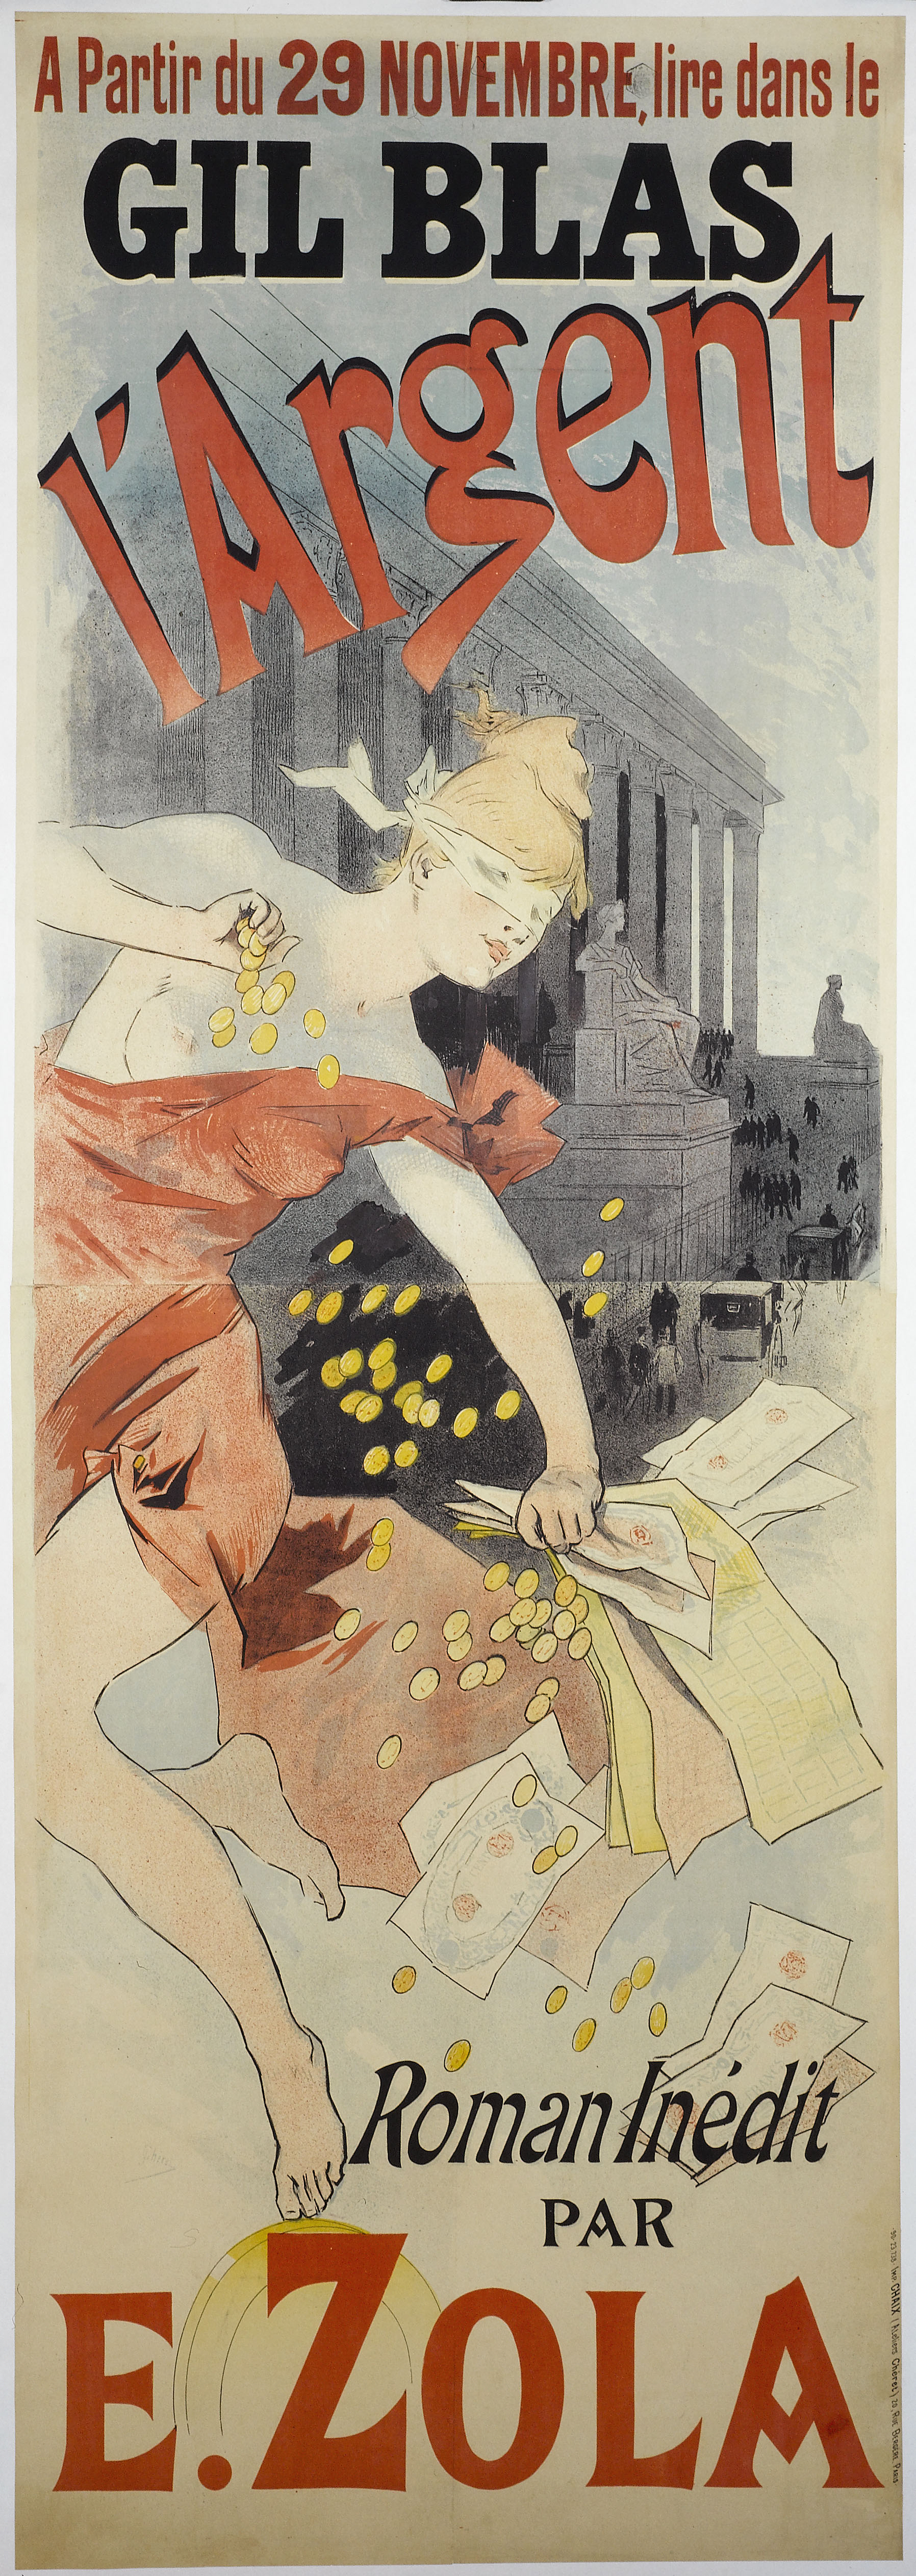
\includegraphics[height=0.63\textheight]{includes/argent.jpg}
				\end{center}
				\\
				\emulatecaption{Alcide Joseph Lorentz, \textit{Monument à Robert Macaire},1856, musée Carnavalet}
			\end{tabular}
		\end{column}
	\end{columns}
\end{frame}	

\begin{frame}{Aborder un quartier par le lieu}{Un cas d'étude: le magasin de nouveautés}
	\begin{columns}[c]
		\begin{column}{0.5\textwidth}
			\begin{tabular}{p{\textwidth}}
				\begin{center}
					\includegraphics[width=0.9\textwidth]{includes/vdf1.png}
				\end{center}
				\\
				\emulatecaption{\textit{\enquote{Aux villes de France}, n° 51 rue Vivienne, n° 104 rue Richelieu, \enquote{magasin de nouveautés le plus vaste de l’univers}}, Bibliothèque historique de la ville de Paris}
			\end{tabular}
		\end{column}
		\begin{column}{0.5\textwidth}
			\begin{tabular}{p{\textwidth}}
				\includegraphics[height=0.35\textheight]{includes/vdf2.png}
				\\
				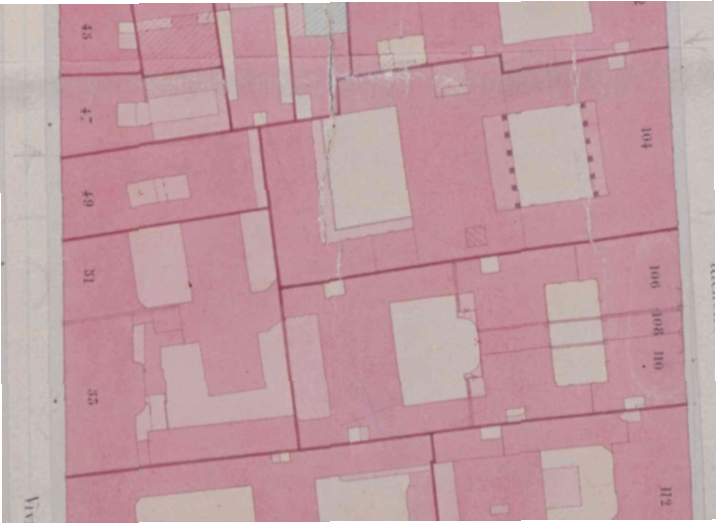
\includegraphics[height=0.35\textheight]{includes/map.png}
				\\
				\emulatecaption{\textit{Plan parcellaire municipal de Paris (fin XIX\textsuperscript{e})}, Quartier Vivienne, Archives de la Ville de Paris}
			\end{tabular}
		\end{column}
	\end{columns}
\end{frame}

\begin{frame}{Aborder un quartier par le lieu}{Spatialiser la ville rêvée}
	\begin{figure}
		\centering
		\begin{subfigure}{0.48\textwidth}
			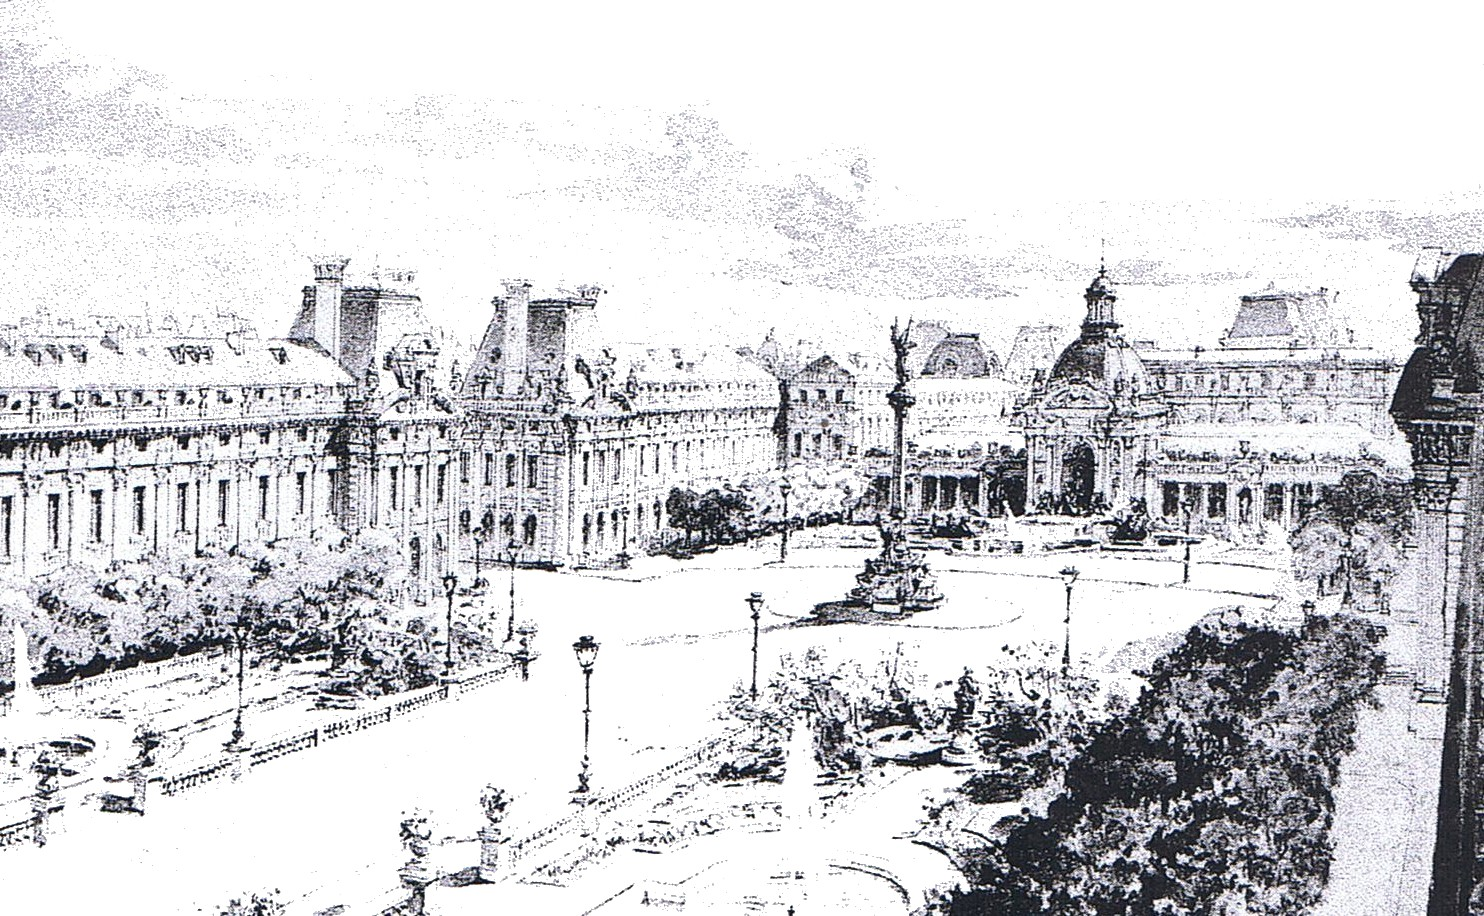
\includegraphics[width=\textwidth]{includes/pr.jpg}
			\caption{Henri Deverin, Projet de transformation du Palais-Royal, \textit{Revue l’architecture}, 1905}
		\end{subfigure}
		\hfill
		\begin{subfigure}{0.5\textwidth}
			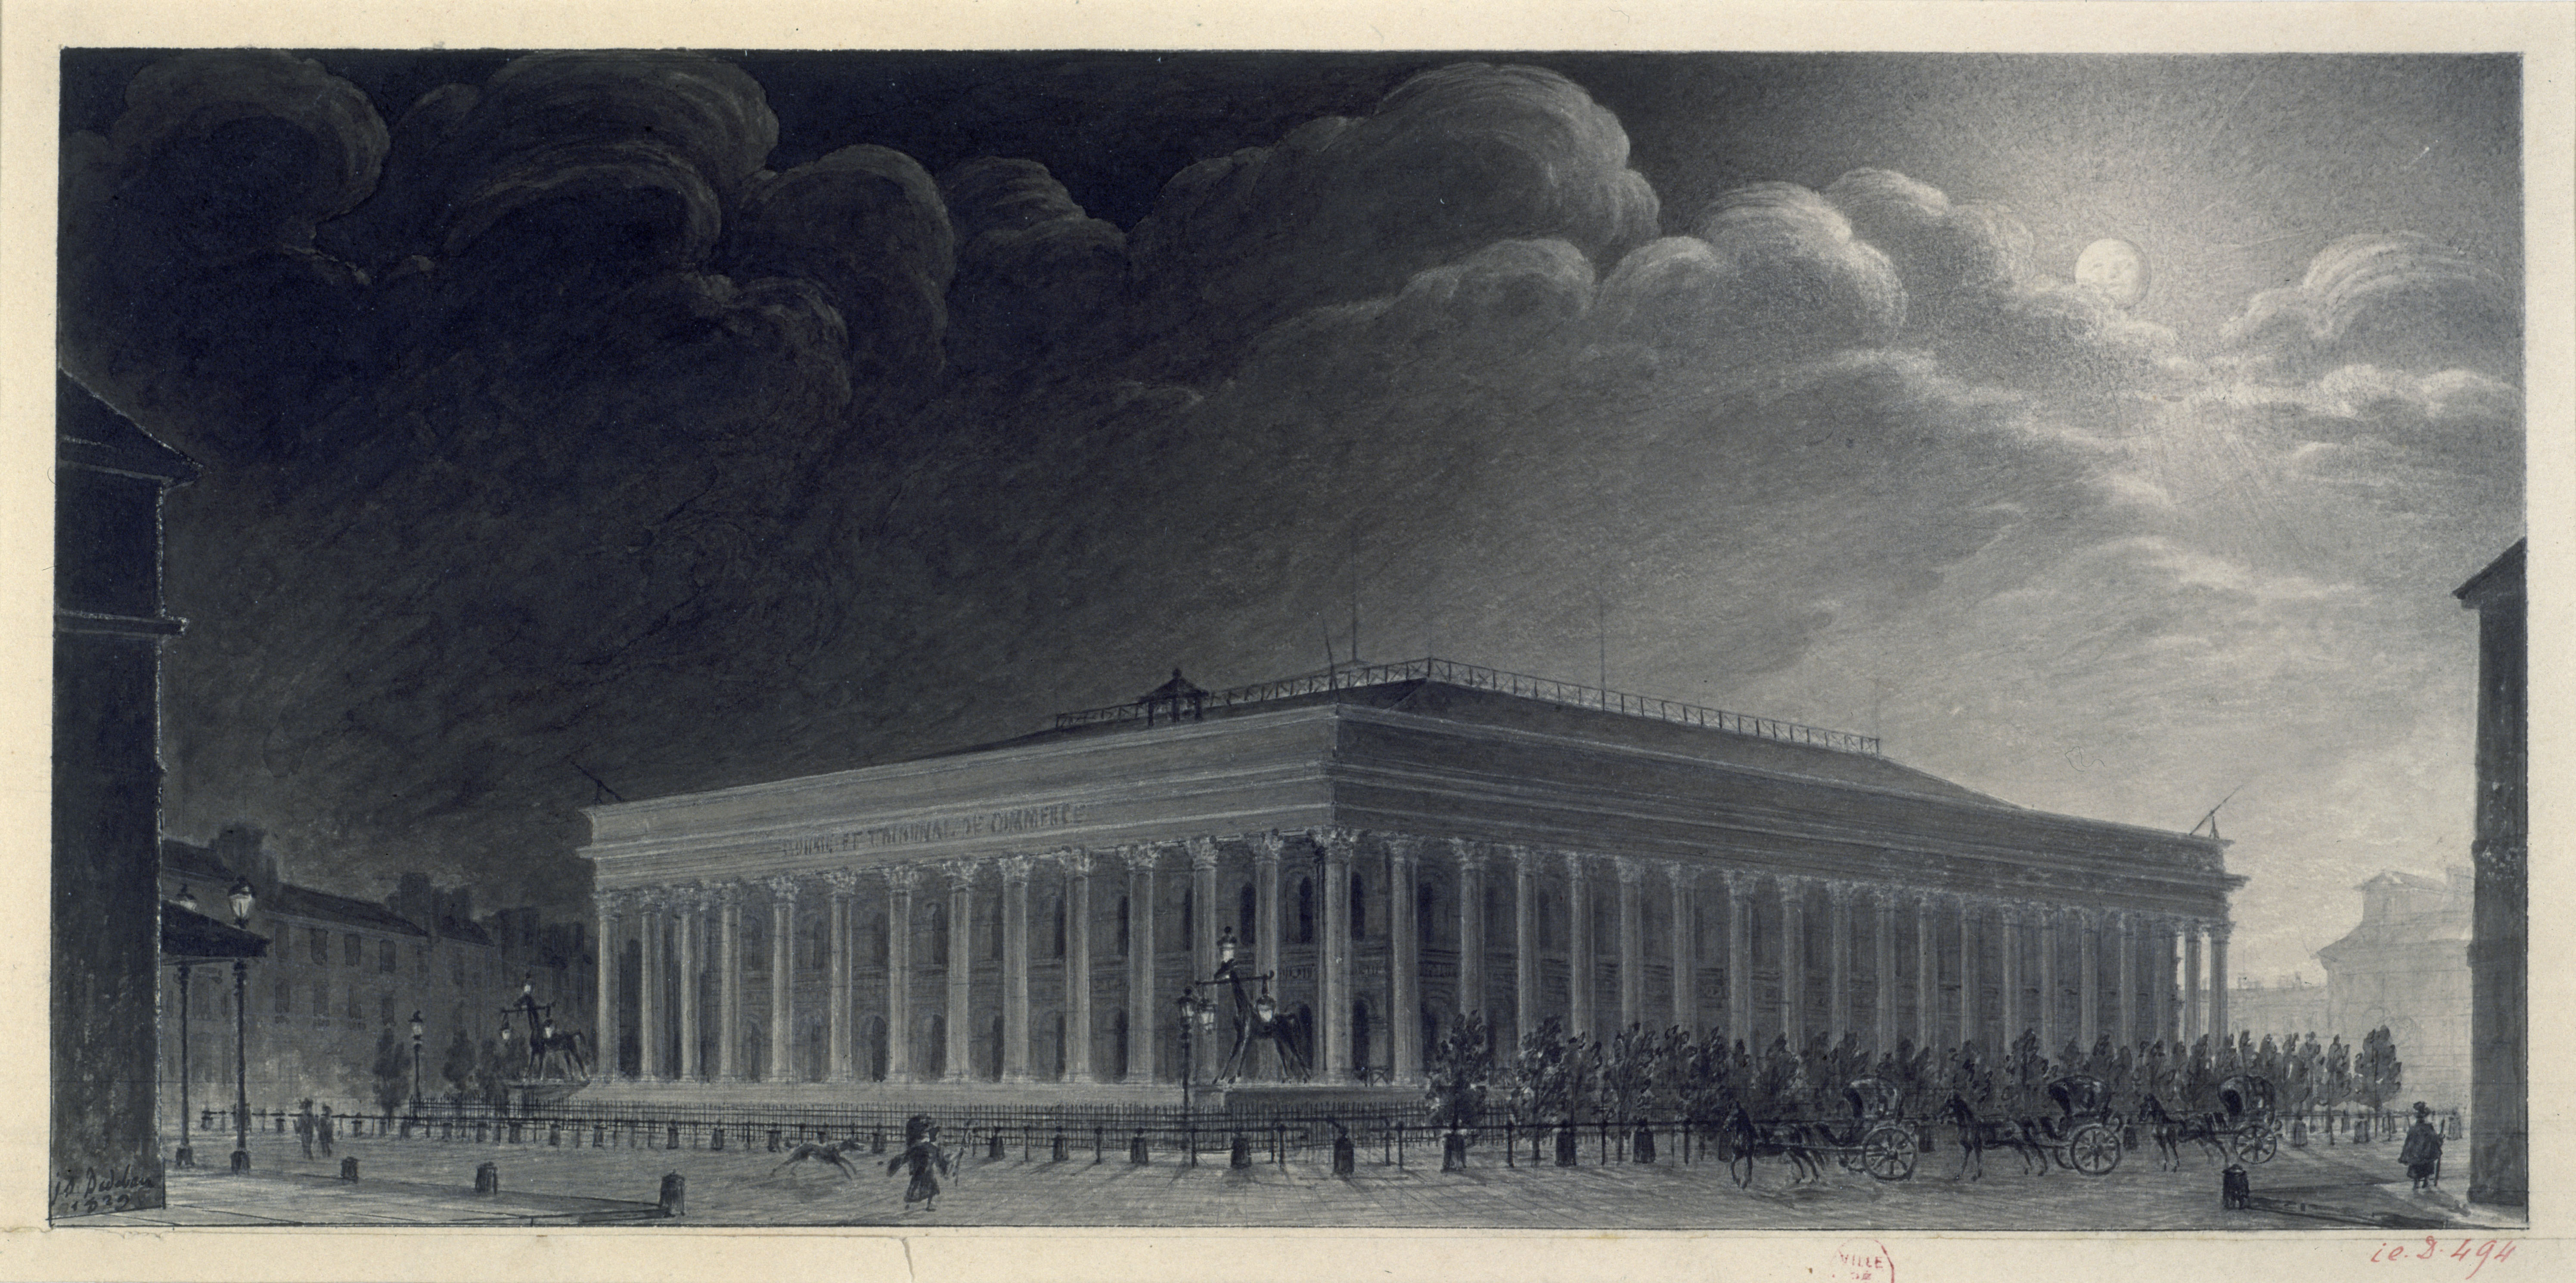
\includegraphics[width=\textwidth]{includes/pb.jpg}
			\caption{Jean-Baptiste Dedeban, \textit{Projet d’éclairage de la Bourse}, musée Carnavalet, 1829}
		\end{subfigure}
		%\hfill
		\begin{subfigure}{\textwidth}
			\centering
			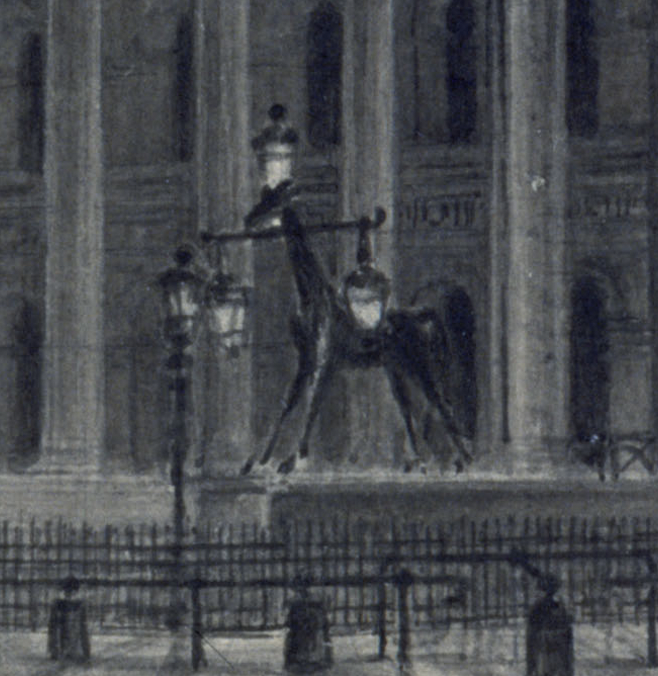
\includegraphics[width=0.25\textwidth]{includes/pb_detail.png}
			\caption{Jean-Baptiste Dedeban, \textit{Projet d’éclairage de la Bourse} (détail), musée Carnavalet, 1829}
		\end{subfigure}
	\end{figure}
\end{frame}

\begin{frame}{Aborder un quartier par le lieu}{Resituer les représentations d'un quartier dans l'espace}
	\begin{figure}
		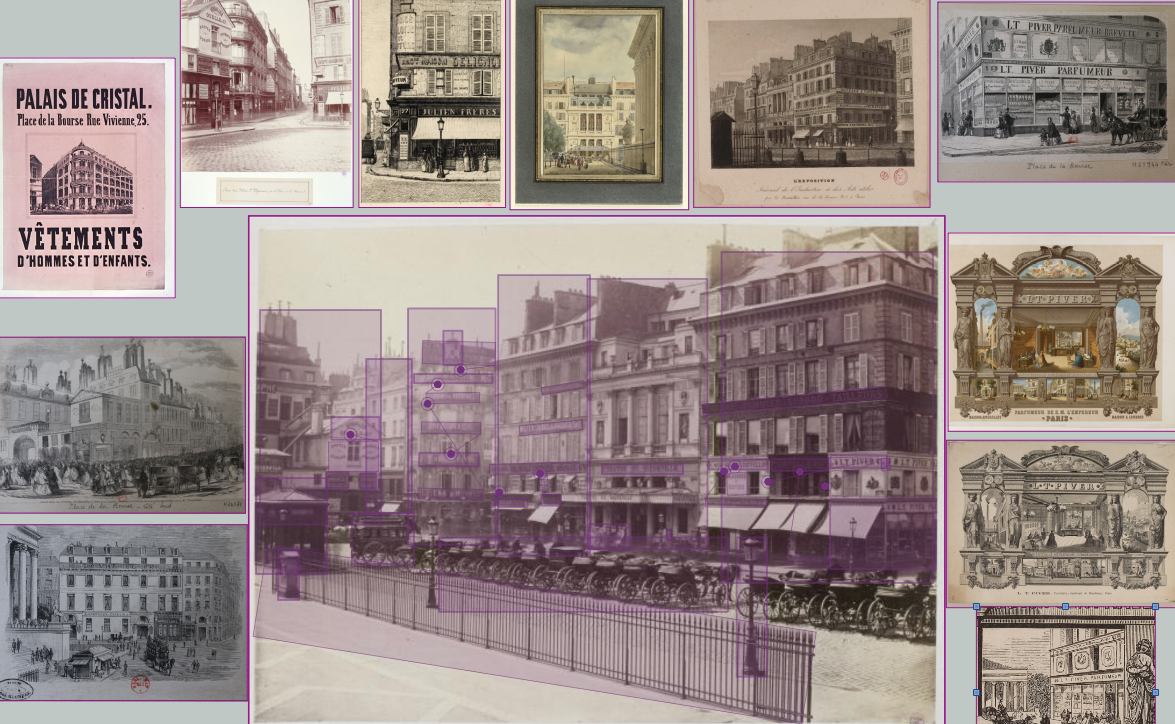
\includegraphics[width=\textwidth]{includes/final_cha.png}
	\end{figure}
\end{frame}

\section{Modéliser un lieu, structurer une pluralité}
\subsection{Une réponse technique à des questionnements théoriques}
\begin{frame}{Modéliser un lieu, structurer une pluralité}{Une réponse technique à des questionnements théoriques}
	Les réflexions sur le lieu \textbf{structurent toute la chaîne de traitement} du projet Richelieu et sont centrales sur \textbf{trois plans}:
	\begin{itemize}
		\item La modélisation des données
		\item La modélisation 3D de la Place de la Bourse
		\item Le développement de l'application Web du projet
	\end{itemize}
	\begin{figure}
		\includegraphics[width=\textwidth]{includes/pipeline-richelieu.png}
		\caption{Chaîne de traitement du projet}
	\end{figure}
\end{frame}


\subsection{Des unités minimales en interrelation: une approche modulaire du lieu}
\begin{frame}{Modéliser un lieu, structurer une pluralité}{Des unités minimales en interrelation: une approche modulaire du lieu}
	Un modèle relationnel (\texttt{SQL}) permet une approche \textbf{modulaire} du lieu:
	\begin{itemize}
		\item Pas du \enquote{sujet} central (contrairement au \texttt{XML})
		\item Le domaine modélisé est divisé en une collection d'objets en interrelation
		\item Plusieurs vues d'un même objet sont possibles
	\end{itemize}
	Le modèle relationnel permet donc de modéliser la complexité du lieu en l'abordant comme un ensemble d'\textbf{unités minimales en interrelation}.
\end{frame}

\begin{frame}{Modéliser un lieu, structurer une pluralité}{Des unités minimales en interrelation: une approche modulaire du lieu}
	\begin{figure}[width=\textwidth,height=\textheight]
		\centering
		\tikz[node distance=1cm, scale=0.7, transform shape]{
			\node[act] (lieu) at (0,0) 
			{
				\tikztemplate{Lieu}{
					\begin{itemize}
						\item Emprise au sol
						\item Durée d'existence (tranche de dates)
					\end{itemize}
				}
			};
		}
		\caption{Modélisation relationnelle d'un lieu}
	\end{figure}
\end{frame}

\begin{frame}{Modéliser un lieu, structurer une pluralité}{Des unités minimales en interrelation: une approche modulaire du lieu}
	\begin{figure}[width=\textwidth,height=\textheight]
		\centering
		\tikz[node distance=1cm, scale=0.7, transform shape]{
			\node[act] (lieu) at (0,0) 
			{
				\tikztemplate{Lieu}{
					\begin{itemize}
						\item Emprise au sol
						\item Durée d'existence (tranche de dates)
					\end{itemize}
				}
			};
			\node[act] (addresse) at (5,0) 
			{
				\tikztemplate{Adresse}{
					Désignation administrative du lieu
					\begin{itemize}
						\item N° de rue
						\item Nom de rue
					\end{itemize}
				}
			};
			\draw[arrow] (lieu) -- (addresse);
		}
		\caption{Modélisation relationnelle d'un lieu}
	\end{figure}
\end{frame}

\begin{frame}{Modéliser un lieu, structurer une pluralité}{Des unités minimales en interrelation: une approche modulaire du lieu}
	\begin{figure}[width=\textwidth,height=\textheight]
		\centering
		\tikz[node distance=1cm, scale=0.7, transform shape]{
			\node[act] (lieu) at (0,0) 
			{
				\tikztemplate{Lieu}{
					\begin{itemize}
						\item Emprise au sol
						\item Durée d'existence (tranche de dates)
					\end{itemize}
				}
			};
			\node[act] (addresse) at (5,0) 
			{
				\tikztemplate{Adresse}{
					Désignation administrative du lieu
					\begin{itemize}
						\item N° de rue
						\item Nom de rue
					\end{itemize}
				}
			};
			\node[act] (carte) at (0,-3) 
			{
				\tikztemplate{Cartographie}{
					Représentation cartographique du lieu dans un document d'archives
					\begin{itemize}
						\item Cartel muséographique
						\item Lien le fichier image spatialisé dans un SIG
					\end{itemize}
				}
			};
			\draw[arrow] (lieu) -- (addresse);
			\draw[arrow] (lieu) -- (carte);
		}
		\caption{Modélisation relationnelle d'un lieu}
	\end{figure}
\end{frame}

\begin{frame}{Modéliser un lieu, structurer une pluralité}{Des unités minimales en interrelation: une approche modulaire du lieu}
	\begin{figure}[width=\textwidth,height=\textheight]
		\centering
		\tikz[node distance=1cm, scale=0.7, transform shape]{
			\node[act] (lieu) at (0,0) 
			{
				\tikztemplate{Lieu}{
					\begin{itemize}
						\item Emprise au sol
						\item Durée d'existence (tranche de dates)
					\end{itemize}
				}
			};
			\node[act] (addresse) at (5,0) 
			{
				\tikztemplate{Adresse}{
					Désignation administrative du lieu
					\begin{itemize}
						\item N° de rue
						\item Nom de rue
					\end{itemize}
				}
			};
			\node[act] (carte) at (0,-3) 
			{
				\tikztemplate{Cartographie}{
					Représentation cartographique du lieu dans un document d'archives
					\begin{itemize}
						\item Cartel muséographique
						\item Lien le fichier image spatialisé dans un SIG
					\end{itemize}
				}
			};
			\node[act] (icono) at (-5,0) 
			{
				\tikztemplate{Iconographie}{
					Ressource iconographique représentant du lieu
					\begin{itemize}
						\item Cartel muséographique
						\item Lien vers des manifestes IIIF pour accéder aux images
					\end{itemize}
				}
			};
			\draw[arrow] (lieu) -- (addresse);
			\draw[arrow] (lieu) -- (carte);
			\draw[arrow] (lieu) -- (icono);
		}
		\caption{Modélisation relationnelle d'un lieu}
	\end{figure}
\end{frame}

\begin{frame}{Modéliser un lieu, structurer une pluralité}{Des unités minimales en interrelation: une approche modulaire du lieu}
	\begin{figure}[width=\textwidth,height=\textheight]
		\centering
		\tikz[node distance=1cm, scale=0.7, transform shape]{
			\node[act] (lieu) at (0,0) 
			{
				\tikztemplate{Lieu}{
					\begin{itemize}
						\item Emprise au sol
						\item Durée d'existence (tranche de dates)
					\end{itemize}
				}
			};
			\node[act] (addresse) at (5,0) 
			{
				\tikztemplate{Adresse}{
					Désignation administrative du lieu
					\begin{itemize}
						\item N° de rue
						\item Nom de rue
					\end{itemize}
				}
			};
			\node[act] (carte) at (0,-3) 
			{
				\tikztemplate{Cartographie}{
					Représentation cartographique du lieu dans un document d'archives
					\begin{itemize}
						\item Cartel muséographique
						\item Lien le fichier image spatialisé dans un SIG
					\end{itemize}
				}
			};
			\node[act] (icono) at (-5,0) 
			{
				\tikztemplate{Iconographie}{
					Ressource iconographique représentant du lieu
					\begin{itemize}
						\item Cartel muséographique
						\item Lien vers des manifestes IIIF pour accéder aux images
					\end{itemize}
				}
			};
			\node[act] (groupe) at (0,2.5) 
			{
				\tikztemplate{Groupement de lieux}{
					Groupement synchronique des évolutions d'un lieu dans le temps
				}
			};
			\draw[arrow] (lieu) -- (addresse);
			\draw[arrow] (lieu) -- (carte);
			\draw[arrow] (lieu) -- (groupe);
			\draw[arrow] (lieu) -- (icono);
		}
		\caption{Modélisation relationnelle d'un lieu}
	\end{figure}
\end{frame}

\begin{frame}{Modéliser un lieu, structurer une pluralité}{Des unités minimales en interrelation: une approche modulaire du lieu}
	\begin{figure}[width=\textwidth,height=\textheight]
		\centering
		\includegraphics[width=0.9\textwidth]{includes/data-model.png}
		\caption{Modèle relationnel complet de la base de données Richelieu}
	\end{figure}
\end{frame}

\subsection{Modélisation partielle et angles morts}
\begin{frame}{Modéliser un lieu, structurer une pluralité}{Modélisation partielle et angles morts}
	Notre approche du lieu est pragmatique et laisse des angles morts:
	\begin{itemize}
		\item Contraintes techniques
		 \item Espace bidimensionnel
	\end{itemize}
\end{frame}

\end{document}